% Created 2021-05-30 Sun 17:24
% Intended LaTeX compiler: pdflatex
\documentclass[a4paper, openany]{book}
\usepackage[utf8]{inputenc}
\usepackage[T1]{fontenc}
\usepackage{graphicx}
\usepackage{grffile}
\usepackage{longtable}
\usepackage{wrapfig}
\usepackage{rotating}
\usepackage[normalem]{ulem}
\usepackage{amsmath}
\usepackage{textcomp}
\usepackage{amssymb}
\usepackage{capt-of}
\usepackage{hyperref}
\input{baseHeader.tex}
\titel{\textbf{Bachelorproject}} \undertitel{Cryptographic library for FPGA's} \opgave{Bachelor Project} \forfatter{Jacob Herbst(mwr148), Jonas Flach Jensen (sjm233)} \dato{12 june 2021} \vejleder{Advisor: Kenneth Skovhede}
\date{}
\title{}
\begin{document}

\maketitle

\begin{abstact}
abstrct
\end{abstract}

\tableofcontents
\listofillustrations

\chapter{Introduction}
\label{sec:org80f6ae5}

\chapter{Background}
\label{sec:org9facd76}
This chapter will present the theoretical aspect applied in implementing our cryptographic library. Firstly, we will briefly give a high-level overview of the target device, Field Programmable Gate Array, followed by an introduction to the programming model which has enabled us to implement the cryptographic functions included in the library. A review of the different cryptographic terms and constructs used in the library is presented for good measure.

The algorithm of the four cryptographic functions in the library is presented in detail in the following order: MD5, SHA256, AES, and ChaCha20.

\section{Field Programmable Gate Arrays}
\label{sec:org99db96a}
Field Programmable Gate Array (FPGA) is an integrated circuit that can be reconfigured in the ``field''. It stands as the opposite of an Application Specific Integrated Circuit (ASIC), which will have a single purpose, whereas FPGA's can be reprogrammed to have different purposes. It means that an FPGA can be configured to work as a CPU, a GPU, or something else entirely. This can be done in Hardware Description Languages such as Verilog or Very High-Speed Integrated Circuit Hardware Description Language (VHDL) and typically run through a program to synthesize the design on the FPGA.
FPGA's consist of a set of Configurable Logic Gates (CLBs) and interconnects between these. CLBs are the reason FPGA's are reprogrammable. They differ from classic logic gates as NAND and such, used in a CPU, since they are constructed by look up tables, which can be reprogrammed, instead of fixed gates. Since these lookup tables can be built for specific purposes, an FPGA can be programmed to do one thing and do it well. This lack of generality is often suitable for both performance and power consumption, compared to a CPU, which needs to be able to do general processing and thus, in general, has more waste.

\section{Synchronous Message Exchange}
\label{sec:SME}
Synchronous Message Exchange (SME) is a programming model to enable FPGA development for software programmers using high-level languages. SME is based on Communicating Sequential Processes (CSP) and at its core constructs from said process calculi, making use of the elements which has proven useful in hardware design\cite{sme}. Using the following concepts from the CSP model\cite{CSP}, SME can be derived:

\begin{itemize}
\item A program consists of a set of named processes.
\item Each process runs concurrently with no form of sharing with other processes.
\item Concurrent processes can communicate using message passing.
\end{itemize}

SME has a similar notion of processes. There exist two types of SME processes, \texttt{simple process} and a \texttt{simulation process}. Of these, the simple process corresponds to a process in CSP as described above. Each simple process in SME will only share communication channels and constants with the other processes. Simple processes will consist of a set of input and output busses, an \texttt{onTick} function, which will run on every clock tick, and a set of optional variables and functions. Since the model revolves around mapping to hardware, every construct inside a simple process should have a fixed size, which means no dynamic lists, while-loops, etc. On the other hand, simulation processes will not be a part of the actual hardware design, making dynamic constructs legal. Furthermore, simple processes have an optional property \texttt{Clocked Process} which means the process will be triggered in parallel with all the other clocked processes at every clock tick, whereas non clocked processes first will be triggered when all processes it depends on is finished.
For the communications channels, SME extends the concepts from CSP by using buses. Instead of using explicit naming for sources and destinations, each process will consist of a set of input and output busses that it can read and write to, respectively. Furthermore, these buses use broadcasting as means of synchronization instead of the blocking non-buffered approach.  The broadcasting happens every clock cycle on the internal clock.
A bus is essentially just a collection of fields that can be read and written depending on the process's access, merely a data transfer object. Thus a simple (and pointless) process that adds two numbers might have two input busses X\{valid,x\} and Y\{valid,y\}. Inside the \texttt{onTick} function, which will be run every tick of the internal clock of SME, could then add the two values x and y if their valid fields were set to true and write the result to a bus RES\{valid, res\}. It is worth noting that a process should not necessarily have one and possibly multiple ``valid''-flags which shows if there is any data on the bus, but this is common in cases where the processes communicate using the ready/valid handshake, for instance, the one specified by the AXI protocols\footnote{AXI ref}, which is the process communications protocol we will be using. It is easy to see how an SME model can be transformed into a dependency graph with processes being nodes and buses the edges. From the dependency graph, it is possible to create an Abstract Syntax Tree (AST) which can be translated into VHDL code\cite{sme}, thus creating the bridge from the high-level model to the low-level hardware implementation. This, in turn, can be fed into a tool such as Xilinx Vivado to synthesize the implementation to actual hardware. For the cryptographic library covered in this report, we will be using the C\# implementation of SME by the models creators\cite{sme}.
\section{A crypto library}
\label{sec:org1a6cf64}
Cryptographic functions are used by developers across most branches, whether communicating securely over a network or hashing programs to do version control.
So there is a motive for having a crypto library for FPGA's. Such a processor has been made before. IBM created their own ``IBM 4758 Secure Coprocessor''\cite{IBM4758}. Another point is modern Hardware Security Modules (HSM) which also do this.
However, the problem with the existing solutions is that many of them require setting up a royalty-based licensing deal, making it difficult to use for experimental development, small projects, research, and academics.
So we set out to create an open-source crypto library.

The crypto library consists of 4 cryptographic functions, two of which are hash functions, MD5 and SHA-256, and two of which are ciphers, AES, and ChaCha.

It should also have an API allowing users to utilize these functions in their projects, as they would with any other library.
These implementations should also be optimized in terms of speed to compete with the existing software solutions.

\subsection{Hashing}
\label{sec:org63abce8}
Hashing is a mathematical concept referring to using a hash function to map some data of arbitrary size to a value of a fixed size. Cryptographic hash functions are a subset of all hash functions.
The reason for this is that for a hash function to be a cryptographic hash function, it needs to uphold several properties to ensure it is secure, such as ensuring that it is hard to find collisions. Computers also have limited space in memory which limits the implementation of hash functions. Lastly and most importantly, computers can't do true randomness.
If a hash function can be implemented with a limited input space, it is pseudo-random, and upholds specific properties listed below, it can be categorized as a ``Cryptographic Hash Function''.
\begin{itemize}
\item It should be deterministic, as the same hash must be computed given the same input.
\item It is unreasonably hard to predict the hashed value. One reason for this is the requirement to exercise the avalanche effect, meaning the tiniest change in the input message would resolve significant changes in the hash.
\item It is collision-resistant, meaning it is unreasonably hard to find two different messages to have the same hash.
\end{itemize}

\textbf{Merkle-Damgård construction}\\
As stated previously, this library includes implementations of MD5 and SHA-256. These are very similar in design and follow a widely known construction method for cryptographic hashing, the Merkle-Damgård construction. One of the reasons this approach is desirable, when developing a cryptographic hashing algorithm, is because the hash function will be collision-resistant given the compression function itself is collision-resistant\footnote{ref to the article}.
From Figure \ref{fig:Merkle} one can see the construction of the hashing function. One can see that the message will be padded to have a certain length since any compression function must work on a fixed size. The compression function \texttt{f} will initially take two arguments, the initialization vector (IV) and the first message block. \texttt{f} will then produce a result of the same size as the initialization vector. This result will then be fed into the next iteration of \texttt{f} and the second block of the message. This process is repeated until the entire padded message has been processed. From here, a potential finalization function can be applied to improve the hash, and a hashed value is hence produced.

\begin{figure}[H]
\centering
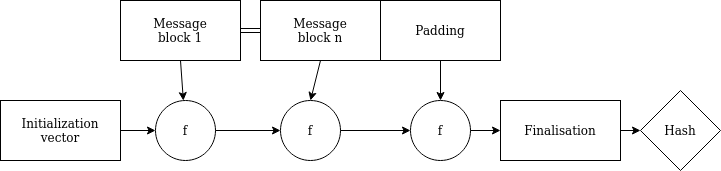
\includegraphics[width=11cm]{merkle.png}
\caption{Merkle-Damgård construction}
\label{fig:Merkle}
\end{figure}
\subsection{Cipher}
\label{sec:org3c293f4}
Ciphers are algorithms used for symmetric encryption and decryption of data. This means that rather than generating a fixed-sized output like most (if not all) hash functions, a cipher should always output as many bits as its input. There are generally two types of ciphers: block ciphers and stream ciphers. They a similar in that they always have to be a bijective mapping from key/plaintext to ciphertext, such that no two plaintexts can map to the same ciphertext. Furthermore, Claude Shannon defined\footnote{ref til confusion difussion} that secures ciphers should have confusion and diffusion. Confusion meaning a bit of the ciphertext should depend on the key in multiple ways, such that no connection between those two is easily observable. Diffusion meaning a single change of bit in the plaintext should change most bits in the ciphertext. For their internal workings, the two types of ciphers are, however, vastly different.\\

\textbf{Block ciphers}\\
Block ciphers are defined to work on a fixed-sized block of bits, which often, and in the case of AES, is 128 bits. This requires some considerations; firstly, data that is not a multiple of the block size will require some type of padding, as the method of choice is not defined by any standard, we have not taken unevenly sized plaintexts into account. To handle data that does not directly fit into a single block multiple Modes of operations are defined. They differ quite a lot in detail, but all conceptually turns the block cipher into a stream. The most simple is Electronic Code Book (ECB), which will independently encrypt each data block. It is worth noting that this is not the most secure mode since identical data blocks will produce identical cipher blocks. Another more secure method is Cipher Block Chaining (CBC), which will xor the previous block's ciphertext with the plaintext of the current block before encrypting the block. This approach is an embarrassingly sequential method. More parallel and secure modes also exist, such as Counter Mode (CTR) and Galois Counter Mode (GCM). These work by taking a nonce as input to the cipher instead of the plaintext. The result will then be XORed with the plaintext. Each block after the initial will then take the nonce increased by some fixed size pr. block.\\

\textbf{Stream ciphers}\\
A stream cipher, as the name suggests, works using stream and is thus independent of size. Stream ciphers generate a pseudorandom keystream, which will be combined with the plaintext. Most often, this combination will be by XOR, such that bit 0th of the plaintext will be XORed with the 0th bit of the keystream.

\section{MD5}
\label{MD5alg}
The Message-Digest algorithm MD5 is a reasonably simple one-way hashing function that produces a 128-bit digest specified in 1992 in RFC 1321\cite{rfc1321}.
The MD5 algorithm will thus create a 128-bit digest from an arbitrary-sized message of n bits. Since MD5 uses a Merkle-Damgård construction, it follows Figure \ref{fig:Merkle}. It will thus partition the n bit message into smaller blocks of 512 bits. This is done by following a fairly common padding scheme, seen in the Merkle-Damgård family. It is done by always padding the message with a single set bit followed by a series of 0's until the message length = 448 mod 512. Thus in situations where the original message has a length of 448 mod 512, a 1 is followed by 511 bits of 0's. Lastly, a Merkle-Damgård strengthening is applied by appending a 64-bit representation of the message length mod 2\textsuperscript{64} to the padded message, resulting in every partition being 512 bits wide.
Each partition of the message will then be fed into the compression \texttt{f} function in Figure \ref{fig:Merkle}.


\begin{figure}[!htb]
\centering
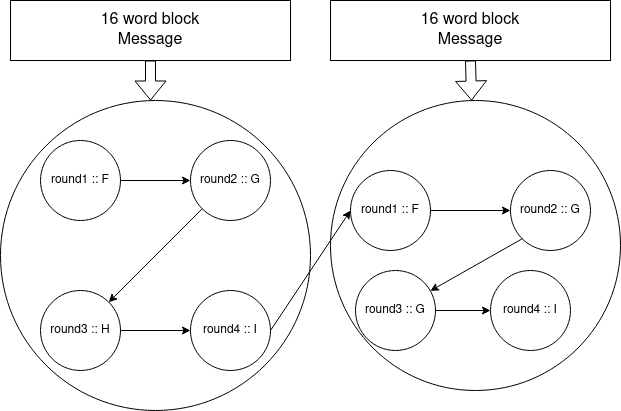
\includegraphics[width=10cm]{MD5rounds.png}
\caption[MD5 Rounds]%
{Rounds of MD5. Each of the two outer circles, is what corresponds to the f-function in Figure \ref{fig:Merkle}. Each of f function consists of a set of functions which will hash the (A,B,C,D) vector and forward it to the next round. The last round of an application of f will forward the vector to the next application of f on the next block of the message.}
\label{fig:MD5}
\end{figure}

Figure \ref{fig:MD5}\footnote{this is a horrible picture and we should prob make a better one} shows the expanded compression function \texttt{f}. \texttt{f} will modify a 128-bit initialization vector (A, B, C, D), with the initial value:\\
\texttt{[} \texttt{A: 0x67542301}, \texttt{B: 0xefcdab89}, \texttt{C: 0x98badcfe}, \texttt{D: 0x10325476} \texttt{]}\\
\texttt{f} will use the following four functions, defined as such, to in ``bitwise parallel'' produce independent and unbiased bits in each of the rounds.
\begin{align}
F(X, Y, Z) &= (X \wedge Y) \vee (\neg X \wedge Z) \\
G(X, Y, Z) &= (X \wedge Z) \vee (Y \wedge \neg Z) \\
H(X, Y, Z) &= X \oplus Y \oplus Z \\
I(X, Y, Z) &= Y \oplus ( X \vee \neg Z)
\end{align}
In \texttt{f} a total number of 64 rounds will be computed, each of the functions 1-4 is applied a total of 16 times. Figure \ref{fig:MD5Rounds} shows each of the specific rounds, where\\
\texttt{[abcd k s i]}\\
denotes \texttt{a = b + (( a + round(b,c,d) + M[k] + K[i]) \textbackslash{}lll s)}, and \texttt{round} denotes the function corresponding to one of the 4 functions corresponding to that round, \texttt{M} denotes the current 16-word buffer of the padded message and \texttt{K[i]} denotes the \texttt{floor(2\textasciicircum{}32 * abs (sin(i + 1)))}.
\begin{table}[!htb]
\centering
\begin{verbatim}
round 1  :: F
[ABCD  0  7  1] [DABC  1 12  2] [CDAB  2 17  3] [BCDA  3 22  4]
[ABCD  4  7  5] [DABC  5 12  6] [CDAB  6 17  7] [BCDA  7 22  8]
[ABCD  8  7  9] [DABC  9 12 10] [CDAB 10 17 11] [BCDA 11 22 12]
[ABCD 12  7 13] [DABC 13 12 14] [CDAB 14 17 15] [BCDA 15 22 16]
Round 2 :: G
[ABCD  1  5 17] [DABC  6  9 18] [CDAB 11 14 19] [BCDA  0 20 20]
[ABCD  5  5 21] [DABC 10  9 22] [CDAB 15 14 23] [BCDA  4 20 24]
[ABCD  9  5 25] [DABC 14  9 26] [CDAB  3 14 27] [BCDA  8 20 28]
[ABCD 13  5 29] [DABC  2  9 30] [CDAB  7 14 31] [BCDA 12 20 32]
Round 3 :: H
[ABCD  5  4 33] [DABC  8 11 34] [CDAB 11 16 35] [BCDA 14 23 36]
[ABCD  1  4 37] [DABC  4 11 38] [CDAB  7 16 39] [BCDA 10 23 40]
[ABCD 13  4 41] [DABC  0 11 42] [CDAB  3 16 43] [BCDA  6 23 44]
[ABCD  9  4 45] [DABC 12 11 46] [CDAB 15 16 47] [BCDA  2 23 48]
Round 4 :: I
[ABCD  0  6 49] [DABC  7 10 50] [CDAB 14 15 51] [BCDA  5 21 52]
[ABCD 12  6 53] [DABC  3 10 54] [CDAB 10 15 55] [BCDA  1 21 56]
[ABCD  8  6 57] [DABC 15 10 58] [CDAB  6 15 59] [BCDA 13 21 60]
[ABCD  4  6 61] [DABC 11 10 62] [CDAB  2 15 63] [BCDA  9 21 64]
\end{verbatim}
\caption{All rounds of a single MD5 iteration}
\label{fig:MD5Rounds}
\end{table}
When all rounds are completed, the new vector (A\textsubscript{1} , B\textsubscript{1} , C\textsubscript{1} , D\textsubscript{1}) will be added to the vector from before the rounds. This result will store the digest for that round. If this results from applying \texttt{f} to the last block of the message, we have the MD5 digest of the message. Is this, however, a result of applying \texttt{f} to any other block, the result will be the IV of the next round.
It is worth noting that MD5 is not a very good hashing algorithm for cryptography, as collision attacks exist, although it uses the Merkle-Damgård construction, but still shows use for data integrity purposes and such.
\section{SHA256}
\label{SHAalg}
SHA256 is a one-way Secure Hash Algorithm, which is where it gets its name from.
It is part of the SHA2 family and was designed and published by the NSA.
SHA256, like MD5, is based upon the Merkle-Damgård construction.

The 256 part refers to the output size of 256 bits.
SHA256 can take input of any size (depending on the implementation) but works
on chunks of 512 bits and then outputs a digest or hash of 256 bits.
Other versions from the SHA2 family exist, like SHA512 and the truncated
versions like SHA224 and SHA384. All of which are very similar.

The SHA256 routine can be expressed as some initialization and then four computation stages.
All of which works on the massage encoded in binary. All operations are also bitwise.

Firstly all constants and variables get initialized. All members of the SHA family use some preset constants for their initial round of calculations.
SHA256 uses an array of size 64, K, consisting of the first 32 bits of the fractional parts of the cube roots of the first 64 prime numbers.
It also uses eight working variables \(H_i\) with an initial value of the first 32 bits of the fractional parts of the square roots of the first 8 prime numbers.
These H variables get updated with each round and contain the final hash after the final round.

Then the message gets padded. In SHA256, the message bit-length needs to be a multiple of 512.
The padding scheme consists of appending a 1 at the end of the message and then appending 0's until the message has a length of \(x*512+448\).
Finally, the length of the original message is appended as a big-endian 64-bit integer.
This also results in SHA256 not being able to handle messages that have a length of over \(2^{64}\).

For the first stage of the computation is to expand the message

As mentioned the input block is of 512 bits, so sixteen 32 bit words. These gets extended to 64 32 bit words.
The extention of the input block works as follows:
\begin{equation}
  W[i] =
  \begin{cases}
    M[i]  &\text{for } 0 \leq i \leq 15\\
    \sigma_1(W_{i-2}) + W[i-16] + \sigma_0(W_{i-15}) + W[i-7] &\text{for } 16 \leq i \leq 63
  \end{cases}
\end{equation}

The second stage is to update the H variables.

The third stage is to compute \(ch\), \(maj\), \(temp_1\) and \(temp_2\) for each of the 64 entries in the array K and the expanded message W.

For the last stage, the H variables get updated one last time, containing the final hash. Then they get appended together and returned.

\begin{figure}[H]
\centering
\includegraphics[width=8cm]{sha-2.png}
\caption{A SHA256 round}
\label{fig:sha256round}
\end{figure}
\section{AES}
\label{AESalg}
The Advanced Encryption Standard (AES) is a symmetric block cipher and specified as the standard for encryption by the National Institute of Standards and Technology (NIST). As AES is the standard for encryption, it is used chiefly everywhere and is critical to include in a cryptographic library. The algorithm behind AES is called Rijndahl and was chosen since it had a good balance of security, performance on a vast variety of devices\cite{AESofficial}. Rijndael is a Substitution-permutation (SP) network that manipulates a block and key size of any multiple of 32 in the range 128-256 bits. In the exact specification of AES, the block size is fixed to 128 bits, where the key potentially can be 128, 192, or 256 bits. The 128 bits are arranged in a 4 x 4 column-major order matrix. As stated, AES is an SP network, meaning it is constructed as a series of rounds of substitutions and permutations. More precisely, the algorithm is listed as follows:
\begin{enumerate}
\item KeyExpansion: The key, whether it be 128, 192 or 256 bits is expanded using a keyschedule which will expand a key into the number of rounds + 1 keys. The schedule look as follows:
\begin{equation*}
W_i \begin{cases}
    K_i & \text{if } i < N\\
    W_{i-N} \oplus \text{SubWords($W_{i-1}\lll 8$))} \oplus \text{rcon}_{i/N} & \text{if } i \geq N \text{ and }  i \equiv 0 (\text{mod } N)}\\
    W_{i-N} \oplus \text{SubWords($W_{i-1}$)} & \text{if $i \geq N$, $N > 6$, and $i \equiv 4$ (mod $N$)}\\
    W_{i-N} \oplus W_{i-1} & \text{otherwise}
\end{cases}
\end{equation*}
where \(i = 0 ... 4 \cdot \text{rounds} - 1\), \(K_i\) is the i\textsuperscript{th} 32 bit word of the original key. \(W\) is a 32-bit word of the expanded key. \(N\) is the number of words in the original key and subword and rcon being defined as follows:
\begin{equation}
 \text{SubWord}([b_0 b_1 b_2 b_3]) = [S(b_0) S(b_1) S(b_2) S(b_3)]
\end{equation}
With \(S\) being the Substitution box explained later for the \texttt{SubBytes} function.
\begin{center}
\begin{tabular}{lrrrrrrrrr}
i & 1 & 2 & 3 & 4 & 5 & 6 & 7 & 8 & 9\\
\hline
rcon\footnote{all values with a trailing 0 bytes} & 01 & 02 & 04 & 08 & 10 & 20 & 80 & 1b & 36\\
\end{tabular}

\end{center}

\item The initial round-key is XORed with the plaintext.
\item SP - round: the rounds of the SP is performed by first doing a substitution which officially is called SubBytes\cite{Rijndael}, followed by the permutation, which consists of 2 functions \texttt{ShiftRows} and \texttt{MixColumns}, which will ensure the 4x4 matrix is permuted and diffused. Lastly, the round-key is XORed with the result. This is done 9, 11, or 13 times depending on whether the key size is 128, 192, or 256 bits, respectively.
\item The last round will work like the other, except it will only permute the rows and not the columns.
\end{enumerate}

Subbytes is a non-linear byte substitution and is usually implemented as a lookup table. It is calculated in 2 steps first by taking the multiplicative inverse in the Galois field GF(2\textsuperscript{8}) followed by an affine transformation over GF(2):
\[b_i = b_i \oplus b_{(i+4) \% 8} \oplus b_{(i+5) \% 8} \oplus b_{(i+6) \% 8} \oplus b_{(i+7) \% 8} \oplus c_i \] with b\textsubscript{i} denoting the i\textsuperscript{th} bit of the byte and c\textsubscript{i} denoting the i\textsuperscript{th} bit of 0x63. Since these and mostly every calculation in AES operates on Galois fields, we can be certain the cipher also will be 128 bits. The lookup table can be seen in Appendix \ref{AESLUT}

ShiftRows will transform the 4x4 input matrix by rotating the rows 0 to 3 bytes to the left, meaning the first row \{b\textsubscript{0}, b\textsubscript{4}, b\textsubscript{8}, b\textsubscript{12}\} will not be rotated, the second row will be rotated one bit to the left, i.e. \{b\textsubscript{5}, b\textsubscript{9}, b\textsubscript{13}, b\textsubscript{1}\} after the rotation. Likewise the 3rd row is shifted 2 and the last row is shifted 3 to the left (or 1 to the right). The transformation can be seen in Figure \ref{fig:ShiftRows}


\begin{figure}[!htb]
\centering
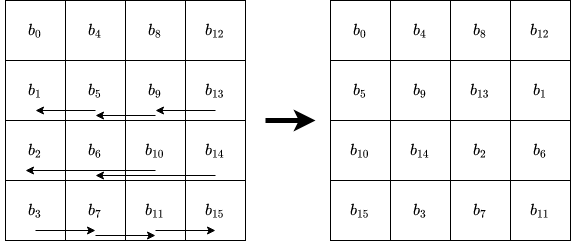
\includegraphics[width=8cm]{shiftRows.png}
\caption[ShiftRows operation]{ShiftRows operation. Shows the rearrangement of the bytes in the matrix}
\label{fig:ShiftRows}
\end{figure}

MixColumns takes each column as a polynomial over the GF(2\textsuperscript{8}) and is multiplied (mod x\textsuperscript{4} +1,as it is a finite field) by \(a(x) = 3x^3 + x^2 + x + 2\), which can be written as a matrix as:
\[
\begin{bmatrix}
 s_{0,c}' \\
 s_{1,c}' \\
 s_{2,c}' \\
 s_{3,c}' \\
\end{bmatrix}=
\begin{bmatrix}
 2 & 3 & 1 & 1 \\
 1 & 2 & 3 & 1 \\
 1 & 1 & 2 & 3 \\
 3 & 1 & 1 & 2 \\
\end{bmatrix}
\begin{bmatrix}
 s_{0,c} \\
 s_{1,c} \\
 s_{2,c} \\
 s_{3,c} \\
\end{bmatrix}
\]
Where c denotes the column, multiplication is as described above, and addition is XOR.

The equivalent inverse functions can be used for decryption, as Rijndael is truly invertible, meaning an implementation in a reversible programming language would result in correct encryption or decryption based on whether the function was called or uncalled.

The original paper for Rijndael\cite{Rijndael} describes how these different steps can be implemented using lookup tables. This implementation can be realized on any 32-bit system with 4096 bits of memory, as we would need 4 lookup tables of 256 32-bit entries. That is one table for each column with all the 256 values in GF(2\textsuperscript{8}). The tables can simply be computed:
\begin{equation}
T_0[a] = \begin{bmatrix}
          S[a] \cdot 02_{16}\\
          S[a]\\
          S[a]\\
          S[a] \cdot 03_{16}
\end{bmatrix}
T_1[a] = \begin{bmatrix}
          S[a] \cdot 03_{16}\\
          S[a] \cdot 02_{16}\\
          S[a]\\
          S[a]
\end{bmatrix}
T_2[a] = \begin{bmatrix}
          S[a]\\
          S[a] \cdot 03_{16}\\
          S[a] \cdot 02_{16}\\
          S[a]
\end{bmatrix}
T_3[a] = \begin{bmatrix}
          S[a]\\
          S[a]\\
          S[a] \cdot 03_{16}\\
          S[a] \cdot 02_{16}\\
\end{bmatrix}
\end{equation}
these will then get used in a round transformation as
\begin{equation}
e_j = T_0 [a_{0,3}] \oplus T_1 [a_{1,2}] \oplus T_2 [a_{2,1}] \oplus T_3 [a_{3,0}] \oplus k_j
\end{equation}
where \(a_{x,y}\) denotes the byte in row \(x\) and column \(y\) and j is the round transformation.

This approach are generally considered faster as it reduces each round to 16 lookups and 16 XORs compared to the normal approach where memory needs to be moved around. This is approach however is more prone to cache timing attacks and since the introduction of AES instruction set in 2010 this method is no longer the fastest on CPUs.
\section{ChaCha20}
\label{ChaChaalg}
ChaCha20 (From hereon just called ChaCha) is a stream cipher intended to be a fast and efficient standby cipher in case AES is compromised. Unlike block ciphers, such as AES, which works on a fixed-sized block of text, stream ciphers work on a per-byte level. This is usually done by combining the plaintext with a pseudorandom stream of digits using XOR. Since the objective of the cipher is to generate a random stream, one first needs a seed. The seed of ChaCha is 16 32 bit words, laid out as such:

\begin{figure}[!htb]
\centering
\includegraphics[width=3cm]{ChaChaSeed.png}
\caption{Seed of ChaCha20}
\label{fig:ChaChaSeed}
\end{figure}

As one can see, the layout of the seed is relatively simple and constitutes 4 parts:
\begin{itemize}
\itemsep 0em
\item A 4 word constant "expand 32-byte k", which is a classic case of a "nothing up my sleeve number".
\item A 256 bit key in little-endian order.
\item A word for the block counter (BC). This is sufficient for up to 256GB of plaintext.
\item A nonce which spans 3 words in little-endian.
\end{itemize}
It might seem counter-intuitive that the seed would include a word, which holds the current block number. However, the result of each iteration of ChaCha20 will result in 16 words generated for the stream. Since the rest of the seed will stay the same for the entire encryption, the increasing block counter will ensure that no two ``blocks'' should result in the same cipher, and essentially including the CTR mode of operation for block ciphers into the streaming cipher. The confusion part of the algorithm follows a simple add-rotate-XOR (ARX) structure. Every round is based on only simple arithmetic add, left rotations, and XOR operations. More specifically ChaCha20 consist of 20 round of which each consist of 4 quarter rounds will confuse 4 input words. Each quarter round looks as shown in Figure \ref{fig:ChaChaQR}
\begin{figure}[H]
\begin{minipage}{0.4\textwidth}
\begin{verbatim}
a += b; d ^= a; d <<<= 16;
c += d; b ^= c; b <<<= 12;
a += b; d ^= d; d <<<= 8;
c += d; b ^= c; b <<<= 7;
\end{verbatim}
\end{minipage}
\qquad
\begin{minipage}{0.4\textwidth}
\includegraphics[width=6cm]{ChaChaQR.png}
\end{minipage}
\caption{ChaCha20 Quarter Round}
\label{fig:ChaChaQR}
\end{figure}
ChaCha will perform 20 rounds consisting of 4 quarter rounds. For a quarter-round (QR) in an even-numbered round it will take a column of the seed as the input, an odd-numbered round will work on diagonals.
\begin{figure}[H]
\centering
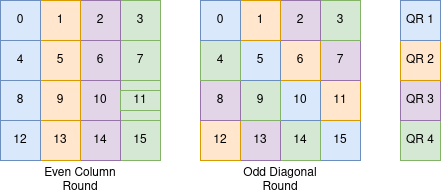
\includegraphics[width=8cm]{diagonal.png}
\caption{ChaCha20 Rounds}
\label{fig:ChaChaRound}
\end{figure}

Lastly, when the 20 rounds have been computed, the initial seed and the modified version are index-wise added, giving a resulting block of 16 words of the stream, and this stream can then be XORed with the plaintext to get the plaintext cipher.

\chapter{Implementation}
\label{sec:orgabed927}
This chapter will go over the implementation-specific details of the algorithms described in the previous chapter. The implementation details will mainly be focused on the usage of SME and how we can structure the algorithms using the different components of SME, to get a working FPGA solution. We describe these implementations first by its naive model, followed by how we can structure a pipeline to improve the performance of each algorithm. We do not explain how the generated VHDL code gets routed to hardware, and we do not describe any interface to use the FPGA from an actual program.

We will be using the streaming AXI protocol (from hereon, just called AXI) for all implementations. AXI is a lightweight protocol for synchronizing data transactions between hardware components. It specifies some standards for a ready/valid handshake between components. This means that whenever a Master component is valid to send data over a bus, and the slave is ready to receive data simultaneously, a transaction is completed. This should ensure that the FPGA version should work with a potential callable interface.
\section{MD5}
\label{sec:org2a7ed17}
\subsection{naive}
\label{MD5naive}
As explained in Section \ref{sec:SME}, SME consists of busses and processes. We can define the MD5 algorithm naively using 4 busses and one simple process.\\

The compression function itself is wholly contained in the single clocked process and works as described in \ref{MD5alg}. The significant difference comes in the data flow. Since our program will be mapped to hardware, we cannot have variable sizes; everything must be static. Thus we have opted for an approach that will receive 512 bits, corresponding to a single message block of the entire message, over the \texttt{Message} which we describe later. The process will both handle the padding and the compression and thus stand as an ``independent'' bus having np dependency on external computations.

For the bus interface between the simulation process and the MD5 process, we considered two overall approaches,
Firstly, one could have 2 input buses to the process, one which would contain the message and one which would contain the IV to modify. However, we find this approach unnecessary as the initialization vector is fixed for every hash, thus the alternative. Since we use the C\# implementation of SME, we can easily store the Digest locally inside the process as a field. We will only require a single data bus with the message. We can define the Message bus as such:
\begin{verbatim}
public interface IMessage : IBus {
    [InitialValue(false)] bool Valid { get; set; }

    [FixedArrayLength(MAX_BUFFER_SIZE)]
    IFixedArray<byte> Message { get; set; }

    int BufferSize { get; set; }
    int MessageSize { get; set; }

    [InitialValue(true)] bool Last { get; set; }
    [InitialValue(true)] bool Head { get; set; }
    [InitialValue(false)] bool Set { get; set; }
}
\end{verbatim}
One can see there are multiple things to keep track of. First and foremost, all busses we will be working with should have a flag for whether or not a bus has data inside of it since we try to adhere to AXI.  Secondly, A byte array is used to store the message block itself. \texttt{BufferSize} will be updated for every iteration or tick, and denotes how many values in the buffer are set, essentially flag for when the message should be padded. \texttt{MessageSize} will be set in the initial tick and denote the length of the entire message used for the Merkle-Damgård strengthening.
The last 3 flags are used to handle some ``edge-cases''.
Head Denotes that the initialization vector should be reconstructed.
Last is used to denote when a block is the last in the message. The block cannot be filled with more than 447 bits.
Set is used when the initial 1 should be set but where the block is not the last in the message, for instance, when the length of the message is 448.

Since we also need to receive the digest from the process, we also need an output bus. This bus is, however, reasonably uncomplicated. It only consists of a Valid flag and the Hash as an array of 4 32-bit words.

Lastly, we want 2 additional busses to make our design comply with the AXI protocol. This bus will be the most basic of all busses and contain only a single flag to show if the process is ready to receive data. It will thus be wired such that the MD5 process will have an in-going bus to know when it is safe to send the digest to the simulation and an out-going ready bus to let the simulation know when to send the message values.

\subsection{First optimization approach}
\label{sec:orgde51948}
To make the algorithm more efficient, the length of the circuit produced in the VHDL code should be reduced. Meaning we want the simple process to do less. For the initial approach, we can notice that the compression function in MD5 works in rounds. Figure \ref{fig:MD5opt1} shows how the hash function as a whole up can be split up into 5 smaller processes and build a pipeline from this. One process for message formatting and one for each of the 4 rounds. In our actual implementation, we further added 2 processes:
\begin{itemize}
\item A message-converter process between the message formatting and \texttt{round 1 (f)} to convert the message from bytes to unsigned integers.
\item A combiner that does the last addition of the two vectors.
\end{itemize}

\begin{figure}[H]
\centering
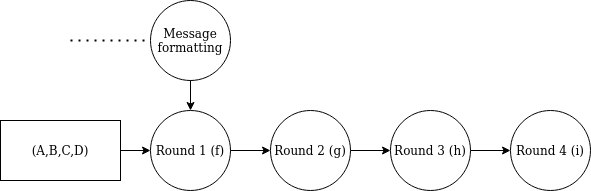
\includegraphics[width=8cm]{md5.png}
\caption[Pipeline MD5]{Highlevel overview of the MD5 pipeline. Each circle is a process and an arrow can be seen as a data bus. The downwards facing arrow carries the initial message and the leftmost arrow is simply (A,B,C,D). All arrows going out from a round carries both (A,B,C,D) and the block.}
\label{fig:MD5opt1}
\end{figure}

However, one problem we have faced with this general approach is that MD5 is embarrassingly sequential because \texttt{round 1 (f)} of the compression of the second message block 2 will depend on the result of \texttt{combiner} of the first message block's compression. This will create a stall. Thus for long messages, the speed-up from the naive version should not be too considerable. However, for tiny messages (<448 bits), the throughput should be noticeably faster as the propagation time should be decreased considerably. As a result of this, we expect to see a possibility to increase the clock frequency, which would trade-off energy use for higher throughput.
As of now, our pipelined versions only work on messages <448 bits.
\subsection{Further optimizations}
\label{sec:org01396f1}
Because the initial optimization approach showed good promise we wanted to see how well a deeper pipeline performed. Hence we further chose to make versions that propagated the rounds into 8, 16, 32, and 64 processes. The results of this can be seen in Section \ref{sec:MD5performance}
\section{SHA256}
\label{sec:orgdd8d5e5}
The implementation of SHA256 is very similar to that of the implementation of MD5,
since they both are hashing algorithms of the Merkle-Damgård construction.
The significant difference is that SHA uses big-endian encodings while MD5 uses little-endian.

\subsection{Naive}
\label{SHAnaive}
The naive unoptimized SHA256 implementation upholds the same general structure in the code, including the padding and block fetching as the naive MD5.
The only difference is that the output digest is 256 bits, so an array of eight 32 bit unsigned integers,
and the format is changed from little-endian to big-endian in the padding and fetch block routines.

So all the busses are set the same and functions the same as in MD5. The exception of the array in the \texttt{Digest} output bus is extended to contain a 256-bit hash.

The SHA256 algorithm is located in the \texttt{processBlock()} routine.
The routine has the input block stored in the first 16 entries of the array \texttt{blockD[]}.
Then these blocks get expanded and the hash calculated as described in Section \ref{SHAalg}.

The calculations for ch, maj, s1, and s0 could be their own functions, but they have been left as written out since they are simple and shouldn't significantly affect performance.
\subsection{Optimizations}
\label{sec:orga3cb99c}
Since SHA256 is so similar to MD5, we can apply the same pipeline approaches as we did for MD5. One difference, however, is the block expansion, which likewise can be pipelined. Thus we should theoretically be able to create an even deeper pipeline for SHA256. Because the target FPGA runs out of resources even before pipelining the rounds, we have not looked into this. The problem and the resource usage will be explained further in Section \ref{sec:SHAperformance}.
\section{AES}
\label{sec:org0a5a67c}

\subsection{Naive}
\label{AESnaive}
Just like for the other algorithms, AES can naively be implemented as a single simple process. That is, we could implement the SME implementation of AES as a single process that can do both encryption and decryption and then have some checks in the \texttt{OnTick} function. This, however, poses some unwanted effects. First, we add unnecessary complications to the process as it would have to multiple things at once. Furthermore, and more importantly, a combined encrypter/decrypter reduces the utilization of the library. Since AES is a block cipher and rarely only needs to encrypt a block of 128 bits, a sequence of blocks needs to be encrypted. This naive approach is not necessarily bad for some of the modes of operations such as Electronic Codebook (ECB) (which never really should be used anyway), Cipher Block chaining (CBC) (which eliminates parallelism), etc. as these will need a decryption algorithm. However, the most used modes: Counter mode (CTR) and Galois-counter mode (GCM), use the encryption algorithm for both encryption and decryption. Thus in a hypothetical scenario where the design includes both encryption and decryption might take up 40 pct. of an FPGA, and a design with only encryption would take up 20 pct. It is clear to see how many resources are wasted. Thus we have decided that for the base case implementation that encryption and decryption should be separate processes. We will only go over the implementation of encryption as the process for decryption is the exact inverse computationally as described in section \ref{AESalg} and the structure thus follows symmetrically. For the design, a single bus with 4 fields, as seen below, suffices. It consists of two Valid flags, which work similarly to the one described for MD5.
Furthermore, there are two-byte arrays with the size of \texttt{BLOCK\_SIZE} = 128 as this implementation is a 128-bit key AES. We have one array for storing the data and one for storing the key. Once again, we don't want to make the process itself flexible with multiple AES versions as it will reduce the resource utilization on an FPGA. This is because the optionality of additional rounds for a 256-bit key version would map these extra computations to hardware, making the circuit more complex and more demanding for Vivado to route the design and have a harder time meeting the timing constraints. In Section \ref{sec:AESperformance} we will take a brief look at this. If 128 key encryption suffices, the overhead from including the 4 extra rounds for 256 is wasteful.

Notice furthermore, the bus is named IPlainText but could just as well have been called IData or something similar as the same bus can be used for both the plaintext and the cipher as the algorithm is symmetrical. However, for the output bus, we don't have to output the key, assuming the result is sent back to the device that called the function.

\begin{verbatim}
public interface IPlainText : IBus {
    [InitialValue(false)]
    bool ValidKey { get; set; }

    [FixedArrayLength(BLOCK_SIZE)]
    IFixedArray<byte> Key { get; set; }

    [InitialValue(false)]
    bool ValidData { get; set; }
    [FixedArrayLength(BLOCK_SIZE)]
    IFixedArray<byte> Data { get; set; }

}
\end{verbatim}
For the actual AES process, we follow the T-box approach described earlier, as we want the throughput of our FPGA to be as efficient as possible despite lacking AES-specific instructions such as \texttt{GF2P8AFFINEINVQB}, \texttt{GF2P8AFFINEQB} and \texttt{GF2P8MULB}.
\subsection{Optimisation 1}
\label{AESopt}
AES has shown to be quite fast even in the naive implementation (see Section \ref{sec:AESperformance}); however, it should still be a reasonably slow approach compared to a pipelined solution, as long as the FPGA can handle the additional logic. Exactly as the other algorithms. We notice that AES likewise uses rounds, and the single process from before can be divided such that each round can is its process. We have tried two solutions this way.

The first solution will merely be the original process split up into smaller parts. This is relatively easy to implement, but it has one flaw which might underutilize the LUT's of the FPGA since each process will only know about each other through a bus and henceforth not have access to the same lookup tables/T-boxes. Corollary, every process that needs access to one of the lookup tables will have to have it defined for itself. Arguably this is a wasteful approach as each process will have to use its own 4KB of T-boxes, which sums up to 36KB. Hence this could be wasteful and use too many LUTs leading to a worse clock rating.

If there are not enough LUTs, we can use the block RAM (BRAM) to our advantage. We can utilize BRAM through SME using \texttt{Components}. To fully utilize the BRAM, we will be using the True Dual Port interface to place multiple T-Boxes in each BRAM without losing utilization. We can further safely do this as we never write to the BRAM, and thus the memory should be as predicted. One thing to be aware of when using BRAM is that it will take 2 clock cycles for a data transaction to happen. With this restriction, there are some considerations to have in mind, should the T-boxes be crammed into a single BRAM, thus having more clock cycles as we can only read a single address at a time, or should we distribute them out on multiple BRAMs to be able to do multiple lookups in each cycle. An approach that would max out the BRAM usage would look as follows:

A single block of the message will include 9 rounds that require 16 lookups. We could arrange the T-Boxes as in Figure\ref{}, with 2 T-boxes in each BRAM. This would not maximize the memory usage as we far from fill the 32 Kbits of memory. But we lose no performance speed-wise. If a single process then has access to two dual ports BRAMs, we would require 18 BRAMs in total for full utilization. \footnote{TODO: this sections should be revised}
\section{ChaCha}
\label{sec:org10e4739}

\subsection{Naive}
\label{ChaChaNaive}
Just like AES, ChaCha will work in two phases. The initial phase will be to set up the seed. After the initial setup, the only modification to the initial seed will be the block counter. We will thus have a similar bus to that of AES. The only difference is that we also need to give the nonce with the input bus. Every iteration will perform ChaCha described in \ref{ChaChaalg}. Like the other algorithms, we have opted for a total solution, meaning the FPGA solution should be as independent as possible. Such that our chacha20 version will not merely produce the keystream but will produce the cipher itself. Thus the input bus should look like this:
\begin{verbatim}
public interface IState : IBus {
    [InitialValue(false)] bool ValidSeed { get; set; }
    [InitialValue(false)] bool ValidT { get; set; }
    uint Nonce0   { get; set; }
    uint Nonce1   { get; set; }
    uint Nonce2   { get; set; }
    [FixedArrayLength(BLOCK_SIZE)]
    IFixedArray<uint> Key { get; set; }
    [FixedArrayLength(TEXT_SIZE)]
    IFixedArray<byte> Text { get; set; }
}
\end{verbatim}
Where \texttt{BLOCK\_SIZE = 16} and \texttt{TEXT\_SIZE = 64}. This design however have posed some challenges.
\subsection{First optimization}
\label{ChaCha1}
version of AES, quite a few table lookups. Furthermore, ChaCha encourages concurrency and parallelism, as each ``block'' can be computed entirely independently of each other in a similar fashion to AES. Thus a pipelined version is easy to implement compared to the has functions. Unfortunately, we have not actually implemented a pipelined option because of the board limitations; the possibility of increasing the performance seemed unreasonable.

\chapter{Results}
\label{sec:orgc34d4b6}
This chapter will go over the performance of the implementations described in the previous chapter. The main focus for our benchmarks has been Throughput and power usage. For comparisons, we settled on similar CPU implementations.
The different implementations have been tested against the C\# standard library equivalent algorithms and ensure that the results are correct. The only exception for this \texttt{ChaCha} as it still is a quite uncommon cipher. All implementations synthesized using Xilinx Vivado on a Zynq Zedboard, which is a low-end FPGA. For comparisons, we have chosen to include different implementations, in C, C\#, and OpenSSL, using \texttt{openssl speed -evp "algorithm"}. Unfortunately, we have not been able to get our hands on the board in time, and we stand with some limitations on the benchmarking results. The reported frequency is the results synthesizing the design through Xilinx Vivado. For comparisons, we settled for a Raspberry pi 4B. The reason being, this having a low-end processor similar to the one on the Zedboard, a Broadcom BCM2711, Quad-core Cortex-A72 (ARM v8) 64-bit SoC @ 1.5GHz. Because of promising results, we further compare our results with an Intel i5-7500.

\section{MD5}
\label{sec:org020a3df}
\label{sec:MD5performance}
\subsection{Throughput}
\label{sec:org0304e93}
\begin{table}[!htb]
\centering
\captionsetup{width=.8\linewidth}
\begin{tabular}{c c c c c c c c}
\hline
Version & f$_{max}$(Mhz) & clocks$_{high}$ & TP(MBps)$_{high}$ & clocks$_{low}$ & TP(MBps)$_{low}$ & LUT & FF\\
\hline
Naive & 2.38 & b & 152.3 & b & 152.3 & 11607 & 2304\\
Proc_{4} & 9.5 &   \( 6+2 \cdot b\) & 265.9 &  \( 2+6 \cdot b\) & 101.3 & 10247 & 5226\\
Proc_{8} & 19 &    \(10+2 \cdot b\) & 531.7 &  \(2+10 \cdot b\) & 121.6 & 10087 & 7538\\
Proc_{16} & 33.5 & \(18+2 \cdot b\) & 937.2 &  \(2+18 \cdot b\) & 119.1 & 10206 & 12162\\
Proc_{32} & 65 &   \(34+2 \cdot b\) & 1816.9 & \(2+34 \cdot b\) & 122.6 &  10149 & 21347\\
Proc_{64} & 115 &  \(66+2 \cdot b\) & 3209.4 & \(2+66 \cdot b\) & 111.5 &  10350 & 39718\\
\end{tabular}
\caption[MD5: FPGA Versions]%
{Performance and statistics over the different MD5 implementations. f$_{max}$ is the clock rate reported from Vivado. Clocks describe how many clock cycles it takes to calculate \texttt{b} blocks, where high and low describe a best and worst-case scenario, respectively. The throughput (TP) is calculated as \((b_{bits}\cdot f_{max})/(clocks \cdot 8)\). LUT is the number of Look-Up Tables used in the design. FF is the reported amount of Flip Flops used. Proc$_{i}$ denotes how many ~i~ processes the 64 rounds are distributed over.}
\label{tab:MD5versions}
\end{table}
As can be seen in Table \ref{tab:MD5versions}, there is a monumental difference between the naive versions. Even the most simple of the pipelines has a 74.6 pct increase over the naive version and the highest performing version, which calculates only a single round in each process more than 20 times faster than the naive version. This comes at the cost of a lot more Flip-Flops but with slightly fewer LUTs. It is, however, quite remarkable that such performance increases are achievable without doing specific FPGA optimizations as such but simply applying pipelining. Especially one aspect has been surprising to see. To keep track of the input block, each process simply forwards it from its input bus to its outputbus. Thus one would assume this computation would take a relatively long time compared to calculating a single round value, but this has not been the case. The reason might be because this is optimized away by Vivado. However, one aspect to be aware of is that the pipelined versions actually ``theoretically'' perform worse than the naive version. The worst case scenario happens when the string to hash is very long as the process thus becomes inherently sequential. Thus the ``cycles saved'' from pipelining will amount to simply 2 cycles, and since the pipelined versions have additional computations, signals, etc., that need to be routed, these will not be as fast as the naive version. Thus if the user need to hash long inputs instead of many short ones, the naive version would be preferable.
\begin{table}[!htb]
\centering
\captionsetup{width=.8\linewidth}
\begin{tabular}{c c c c c c c c}
\hline
\textbf{Version} & Naive & Proc_{64} & C\# & C & C$_{t}$ & OpenSLL$_{low}$ & OpenSLL$_{high}$\\
\hline
\textbf{TP(MBps)} & 152 & 3210 & 287 & 154 & 256 & 42 & 293\\
 & & & 604 & 622 & 600 & 81 & 691
\end{tabular}
\caption[MD5: FPGA and CPU comparisons]%
{Performance comparison of the worst and best MD5 FPGA implementations and the various CPU versions. The C\# uses the \texttt{System.Security.Cryptography.MD5}, the C version and C$_t$ are our implementations and are optimized with \texttt{-O3}. The OpenSSL is from \texttt{openssl speed -evp md5}. Each of the CPU implementations has two values, the first being the Pi results and the second the I5 results.}
\label{tab:MD5compare}
\end{table}
Comparing the implementations to the CPU versions, the naive only perform adequately with the C version on the Pi. Likewise, it seems to beat OpenSSL\textsubscript{low} by quite a margin. The OpenSSL\textsubscript{low} is the worst utilization of the \texttt{openssl speed}, which happens on message sizes of 16 bytes. Compared to the worst utilization of OpenSSL, this is a speedup of more than 300 pct. One should keep in mind that OpenSSL only works on inputs of 16 bytes, which is not nearly enough to fill a block, and thus entire blocks of data are not processed, meaning there is a significant spill. Even when running the same benchmarks on the I5, 16 bytes are merely 81 MB/s. Thus to get the full utilization, we should focus the attention on 256-byte blocks or higher, as the 64-byte blocks will have a round of ``wasteful'' computation as this block is purely padding and not part of the message size.
Compared to all the other CPU versions, the naive version performs poorly, especially on the I5, where most versions are around 4 times faster. On the other hand, the best-performing pipeline outperforms all the CPU versions by a significant amount by at least 4.6 times. This is a significant increase in speed, emphasizing how well an FPGA can perform if designed correctly. However, the Throughput of the optimal pipeline will only serve as the theoretical maximum, and in a real-world example, such speed might not be observable depending on how fast the host can provide the data for the FPGA.
\subsection{Power Consumptions}
\label{sec:org9998a73}
From the previous section, we showed that our FPGA solution could outperform not only low-end CPUs but also mid-end CPUs by quite a margin. But, not only is the FPGA able to achieve high throughput it also does it at very low power consumption. Figure \ref{fig:md5_naive_power} shows the power consumption as reported by Vivado. The power consumption of the naive version sums up to 0.016 watts without including the processing system, which is almost 11 times less than the optimized version using 0.189 watts. Thus, we can see that one needs only 11 times as much power to get a speed increase of 20 times. Interestingly the most of the power usage can be attributed to the clocking.
In any case, we can assume this to be very power efficient compared to the power used by a CPU without having any actual proof of this. We base this assumption that the processing system (PS7) uses at least 88 percent of the power.
\begin{figure}[H]
\centering
\subfloat[Naive version]{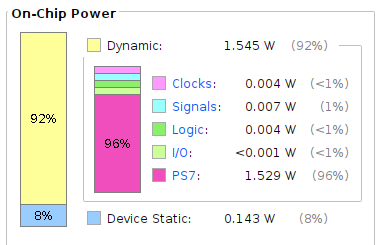
\includegraphics[width=6cm]{MD5_naive_power.png}}
\subfloat[Proc$_{64}$ version]{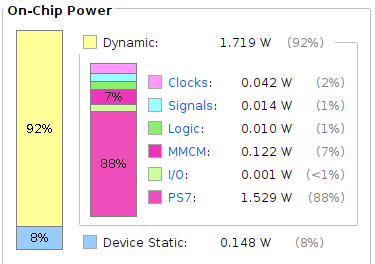
\includegraphics[width=6cm]{MD5_opt_power.png}}
\caption[Power consumption of MD5 designs]%
{Powerconsumption of MD5 designs}
\label{fig:md5_naive_power}
\end{figure}
\subsection{Takeaways}
\label{sec:org83d2f69}
The takeaway from these results is that if one needs to hash long strings, one might as well choose a CPU implementation over our versions, and is one to use our implementations for such one should use the naive version, whereas the pipelined version will be a lot faster (or at least not be the bottleneck). If the power consumption by the computations, on the other hand, is more important than throughput, our naive version is a good alternative over the other implementations presented in the previous sections.
\section{SHA256}
\label{sec:org49a56b8}
\label{sec:SHAperformance}
\subsection{Throughput}
\label{sec:org783e540}
\begin{table}[!htb]
\centering
\captionsetup{width=.8\linewidth}
\begin{tabular}{c c c c c c c c}
\hline
Version & f$_{max}$(Mhz) & clocks$_{high}$ & TP(MBps)$_{high}$ & clocks$_{low}$ & TP(MBps)$_{low}$ & LUT & FF\\
\hline
Naive & 2.1 & b & 134.4 & b & 134.4 & 24330 & 2560\\
Proc_{4} & 8 &   \( 6+2 \cdot b\) & 223.9 &  \( 2+6 \cdot b\) & 85.3 & 24466 & 8938\\
Proc_{8} & 8 &    \(10+2 \cdot b\) & 223.8 & \(2+10 \cdot b\) & 51.2 & X & X\\
\end{tabular}
\caption[SHA256: FPGA Versions]%
{Performance and statistics over the different SHA implementations. f$_{max}$ is the clock rate reported from Vivado. Clocks describe how many clock cycles it takes to calculate \texttt{b} blocks, where high and low describe a best and worst-case scenario, respectively. The throughput (TP) is calculated as \((b_{bits}\cdot f_{max})/(clocks \cdot 8)\). LUT is the number of Look-Up Tables used in the design. FF is the reported amount of Flip Flops used. Proc$_{i}$ denotes how many ~i~ processes the 64 rounds are distributed over.}
\label{tab:SHAversions}
\end{table}
Looking at the statistics in Figure \ref{tab:SHAversions} one can see there is no real difference in Mhz between Proc\(_4\) and Proc\(_8\). This, in turn, means there is a negligible performance difference in a best-case scenario, where many small hashes are calculated. On the other hand, the performance in a worst-case scenario is in favor of Proc\(_4\), since the pipeline of Proc\(_8\) is longer and provides no additional speed because of the serialness. Thus the shorter pipeline Proc\(_4\) should always be considered over any deeper pipeline for boards of similar size to the Zynq. The reason SHA cannot meet the same magnitude of improvement as MD5 is caused by the high usage of LUTs. Compared to MD5, SHA uses around 2.3 times as many LUTs (24466/10350), which makes the routing of the design harder. The additional LUT usage comes from the expanding of the input block from 512 bits to 2048 bits. In any case, the pipelined versions do perform better than the naive version in an optimal scenario, by a 66.5 pct. However, in a worst-case scenario, the naive version is 55.6 pct faster than Proc\(_4\). Thus just as for MD5, the best-suited version will be application-specific.
\begin{table}[!htb]
\centering
\captionsetup{width=.8\linewidth}
\begin{tabular}{c c c c c c}
\hline
\textbf{Version} & Naive & Proc_{4} & C\# & OpenSLL$_{low}$ & OpenSLL$_{high}$\\
\hline
\textbf{TP(MBps)} & 134 & 224 & 163 & 42 & 165\\
 & & & 438 & 61 & 461
\end{tabular}
\caption[SHA256: FPGA and CPU comparisons]%
{Performance comparison of the worst and best SHA FPGA implementations and the various CPU versions. The C\# uses the \texttt{System.Security.Cryptography.SHA256}. The OpenSSL is from \texttt{openssl speed -evp md5}. Each of the CPU implementations has two values, the first being the Pi results and the second the I5 results.}
\label{tab:SHAcompare}
\end{table}
Just as with MD5, the throughput of the naive SHA version is slower than the CPU versions. For the naive SHA version, the naive version is only 30 MBps slower than the CPU versions on the Raspberry Pi, whereas MD5 was only half as fast (difference of 141 MBps). Likewise, the pipelined version performs reasonably well compare to the Pi, with an overall increase of 35.7 pct. Comparing to the I5, the results are not as promising. The pipelined version is only about half as fast as the CPU versions.
\subsection{Power Consumptions}
\label{sec:org931df34}
Figure \ref{fig:SHA_power} shows the power consumption of the naive version and Proc\(_4\). Once again, the results are very similar to those of MD5. The SHA version consumes only about 0.02 watts more than the naive MD5 version. This additional cost is attributed to additional signals and more logic required to compute SHA. Similarly, the pipelined version is a little more power-hungry than MD5. The thing to remember is that the throughput does not follow the same trend.
Interestingly, most of the power consumption of the pipelined MD5 goes towards the clocks, whereas the power consumed by SHA is mainly placed in the computations. This might be because the pipeline is far deeper in MD5. The actual power usage for the two SHA versions is 0.036 watts for the naive version and 0.202 watts for Proc\(_4\), meaning the Proc\(_4\) uses 5.6 times more power, but it only gives a 2-time speedup. Hence, the naive version is more power-efficient than the pipelined version.
\begin{figure}[H]
\centering
\subfloat[Naive version]{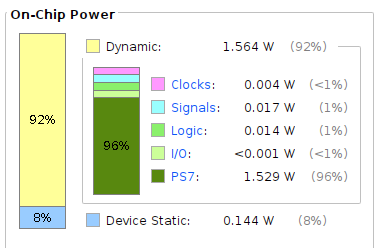
\includegraphics[width=6cm]{SHApower.png}}
\subfloat[Proc$_{4}$ version]{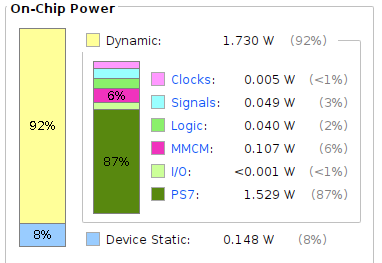
\includegraphics[width=6cm]{SHAopt1power.png}}
\caption[Power consumption of SHA256 designs]
{Powerconsumption of SHA designs}
\label{fig:SHA_power}
\end{figure}
\subsection{Takeaways}
\label{sec:org90d0bdb}
The overall results for SHA are inferior to MD5. The pipelined version could compete with the Raspberry Pi but is still slower than an I5 processor. If power consumption is of concern, the naive version should always be chosen over the pipelined as the throughput increase does not match the increase in power usage.
\section{AES}
\label{sec:orge1cba33}
\label{sec:AESperformance}
\footnote{This section is not done}
\subsection{Throughput}
\label{sec:org0b44bcf}
The results of AES is interesting compared to our other implementations in the sense that even the naive FPGA version is outperforming the CPU. One can notice that our naive version has a throughput of 400 MB/s which is around 4.49 times as much as OpenSLL on its peak performance and that it likewise outperforms C\# and our own C-version with 5.7 and 6.2 times respectively. Even the threaded version is only half as fast as the FPGA solution. These results are quite promising in itself and clearly shows that the FPGA is very suitable for solutions as this one and in cases where large amounts of data needs to be encrypted or decrypted the FPGA is preferable over an arm processor. It is however still worth noting that this still only outperforms processors that does not have AES-NI. For instance running the same OpenSSL benchmark on an intel i7-7500 the worst case has a throughput of 788 MB/s and an optimal solution of 5.61 GB/s. Even though there is a significant price difference between the ARM and Intel processor it still hints to how AES-NI, essentially a dedicated ASIC, outperforms more general CPU solutions by an order of magnitude. One aspect which would have been interesting to measure is how well the implementation synthesized on a high-end FPGA would perform compared to cabable CPU's. An article from 2020 which compares both pipelined and non-pipelined versions of AES on FPGA's shows that even on expensive FPGA's such as the Virtex-7 family only runs between 2.06-6.34 Gbps (257.5-792.5 MB/s)\cite{FPGA_AES}. Thus a nonpipelined version will never be able to compete with an ASIC. One aspect that would have been interested exploring is how well our highlevel version would compare to a solution which has been optimized directly in one of the HDL languages. We have not been able to do this but we can hint at the fact that some of the solutions described previously performs worse than our solution despite the difference in chipset.
\begin{table}[htbp]
\centering
\begin{tabular}{|c|c|c|c|c|c|c|}
\hline
\textbf{Version} & Naive & C\# & C & C\textsubscript{t} & OpenSSL\textsubscript{low} & OpenSSL\textsubscript{high}\\
\hline
\textbf{Throughput} (MB/s) & 400 & 70 & 64.49 & 198.28 & 72.4 & 89.06\\
\hline
\end{tabular}
Benchmarking results for AES.

\end{table}
In the implementation section we described how we rejected to make a solution that was flexible in its key-size. The results hint that this have good impact on the performance. Comparing our solution to the solution presented in the SME github repository, which is more flexible in the key size, our solution outperforms this by a factor of 1.66, as it is reported to have a throughput of 1.92Gbps(240MB/s)\cite{sme}. This shows that we can tradeoff some flexibility for a significant speedup.
\subsection{Power Consumptions}
\label{sec:org95cb41d}

\subsection{Takeaways}
\label{sec:orgbd4e130}
\section{ChaCha20}
\label{sec:org3b2be97}
\footnote{not entirely done}
One would expect ChaCha20 to perform well, because of the simplicity in computation, the fact it was design for speed and that the OpenSSL as reported in Table \ref{tab:ChaChaperformance} is more than 3 times faster than AES as shown in Table \ref{tab:AESperformance}. Despite this, our ChaCha solution cannot even be routed at 1 Mhz, which would correspond to a throughput of merely 64 MBps. This would be almost 5 times slower than OpenSSL on the Raspberry Pi.
\begin{table}[htbp]
\centering
\begin{tabular}{|c|c|c|c|}
\hline
\textbf{Version} & Naive & OpenSSL\textsubscript{low} & OpenSSL\textsubscript{high}\\
\hline
\textbf{Throughput} (MB/s) & ? & 84.03 & 306.81\\
\hline
\end{tabular}
Benchmarking results for Chacha.

\end{table}
The culprit of ChaCha20's poor peformance is the high amount of nets. Nets is sythetic datapath in Vivado, which will be transformed into a wire when mapped to hardware. This suggests that we have too much data on the busses between the interlectual property (IP) and the register transfer level (RTL) of the design. This seems quite a reasonable argument as the input bus itself takes in 1152 bits and the output bus carries 544 bits to output the cipher.
To have a more concrete proof of this we also implemented a version which only generates the keystream, meaning it performs all the quaterrounds but without doing the XOR with the plaintext. This reduces the input and output busses to 610 and 513 bits respectively. When routing the keystream version in Vivado we get a reported frequency of 200 Mhz. Thus there is a huge difference.

\chapter{Discussion}
\label{sec:org7c1394e}
\begin{itemize}
\item SME vs VHDL
\item How easy is FPGA programming
\item ???
\end{itemize}

\chapter{Conclusion}
\label{sec:org2f48346}

\bibliographystyle{unsrt}
\bibliography{ref}

\begin{appendix}
\chapter{AES Look Up Table}
\label{AESLUT}
\begin{table}[!htb]
\centering
\captionsetup{width=.8\linewidth}
\begin{tabular}{c || c c c c c c c c c c c c c c c c}
\hline
   & 00 & 01 & 02 & 03 & 04 & 05 & 06 & 07 & 08 & 09 & 0a & 0b & 0c  & 0d & 0e & 0f\\
\hline
00 & 63 & 7c & 77 & 7b & f2 & 6b & 6f & c5 & 30 & 01 & 67 & 2b & fe  & d7 & ab & 76\\
10 & ca & 82 & c9 & 7d & fa & 59 & 47 & f0 & ad & d4 & A2 & af & 9c  & a4 & 72 & c0\\
20 & b7 & fd & 93 & 26 & 36 & 3f & f7 & cc & 34 & a5 & E5 & f1 & 71  & d8 & 31 & 15\\
30 & 04 & c7 & 23 & c3 & 18 & 96 & 05 & 9a & 07 & 12 & 80 & e2 & eb  & 27 & b2 & 75\\
40 & 09 & 83 & 2c & 1a & 1b & 6e & 5a & a0 & 52 & 3b & D6 & b3 & 29  & e3 & 2f & 84\\
50 & 53 & d1 & 00 & ed & 20 & fc & b1 & 5b & 6a & cb & Be & 39 & 4a  & 4c & 58 & cf\\
60 & d0 & ef & aa & fb & 43 & 4d & 33 & 85 & 45 & f9 & 02 & 7f & 50  & 3c & 9f & a8\\
70 & 51 & a3 & 40 & 8f & 92 & 9d & 38 & f5 & bc & b6 & Da & 21 & 10  & ff & f3 & d2\\
80 & cd & 0c & 13 & ec & 5f & 97 & 44 & 17 & c4 & a7 & 7e & 3d & 64  & 5d & 19 & 73\\
90 & 60 & 81 & 4f & dc & 22 & 2a & 90 & 88 & 46 & ee & B8 & 14 & de  & 5e & 0b & db\\
a0 & e0 & 32 & 3a & 0a & 49 & 06 & 24 & 5c & c2 & d3 & Ac & 62 & 91  & 95 & e4 & 79\\
b0 & e7 & c8 & 37 & 6d & 8d & d5 & 4e & a9 & 6c & 56 & F4 & ea & 65  & 7a & ae & 08\\
c0 & ba & 78 & 25 & 2e & 1c & a6 & b4 & c6 & e8 & dd & 74 & 1f & 4b  & bd & 8b & 8a\\
d0 & 70 & 3e & b5 & 66 & 48 & 03 & f6 & 0e & 61 & 35 & 57 & b9 & 86  & c1 & 1d & 9e\\
e0 & e1 & f8 & 98 & 11 & 69 & d9 & 8e & 94 & 9b & 1e & 87 & e9 & ce  & 55 & 28 & df\\
f0 & 8c & a1 & 89 & 0d & bf & e6 & 42 & 68 & 41 & 99 & 2d & 0f & b0  & 54 & bb & 16
\end{tabular}
\caption[AES]%
{AES Look Up Table, every value is shown in hex}
\label{tab:AESTable}
\end{table}
\end{appendix}
\end{document}
